\section{A Study of Go's \unsafe{} Usages in the Wild}
\label{sec:eval}


We designed and performed a study of Go \unsafe{} usage to answer the following research questions:

\begin{enumerate}[leftmargin=*,label={RQ\arabic*}]
    \item How prevalent is \unsafe{} in Go projects? \label{rq:prevalApp}
    \item How deep are \unsafe{} code packages buried in the dependency tree? \label{rq:depsDepth}
    \item Which \unsafe{} keywords are used most? \label{rq:distTypes}
    \item Which \unsafe{} operations are used in practice, and for what purpose? \label{rq:purpose}
\end{enumerate}

%Figure~\ref{fig:study-overview} provides an overview of our study methodology.
%\begin{figure}[ht]
    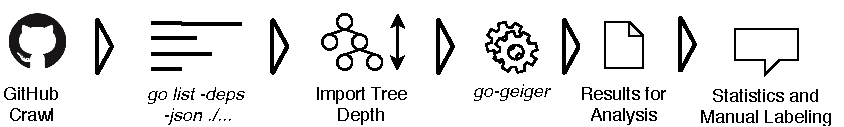
\includegraphics[width=\textwidth]{assets/figures/study-methodology.pdf}
    \caption{Overview of our Study Methodology}
    \label{fig:study-methodology}
\end{figure}


In the following, we first describe our evaluation data set and then provide in-depth analyses of \unsafe{} usage in the wild using \toolUsage{}.
% of how prevalent \unsafe{} is in the wild, in which way and why it is used in our test data set.
Our evaluation scripts as well as the results are available online\footnote{\url{https://github.com/stg-tud/unsafe_go_study_results}}.
%for further research.


%% included here for manual positioning one page earlier. Belongs to next section, reposition if needed
\begin{figure*}[!t]
    \vspace{2mm}
    \centering
    %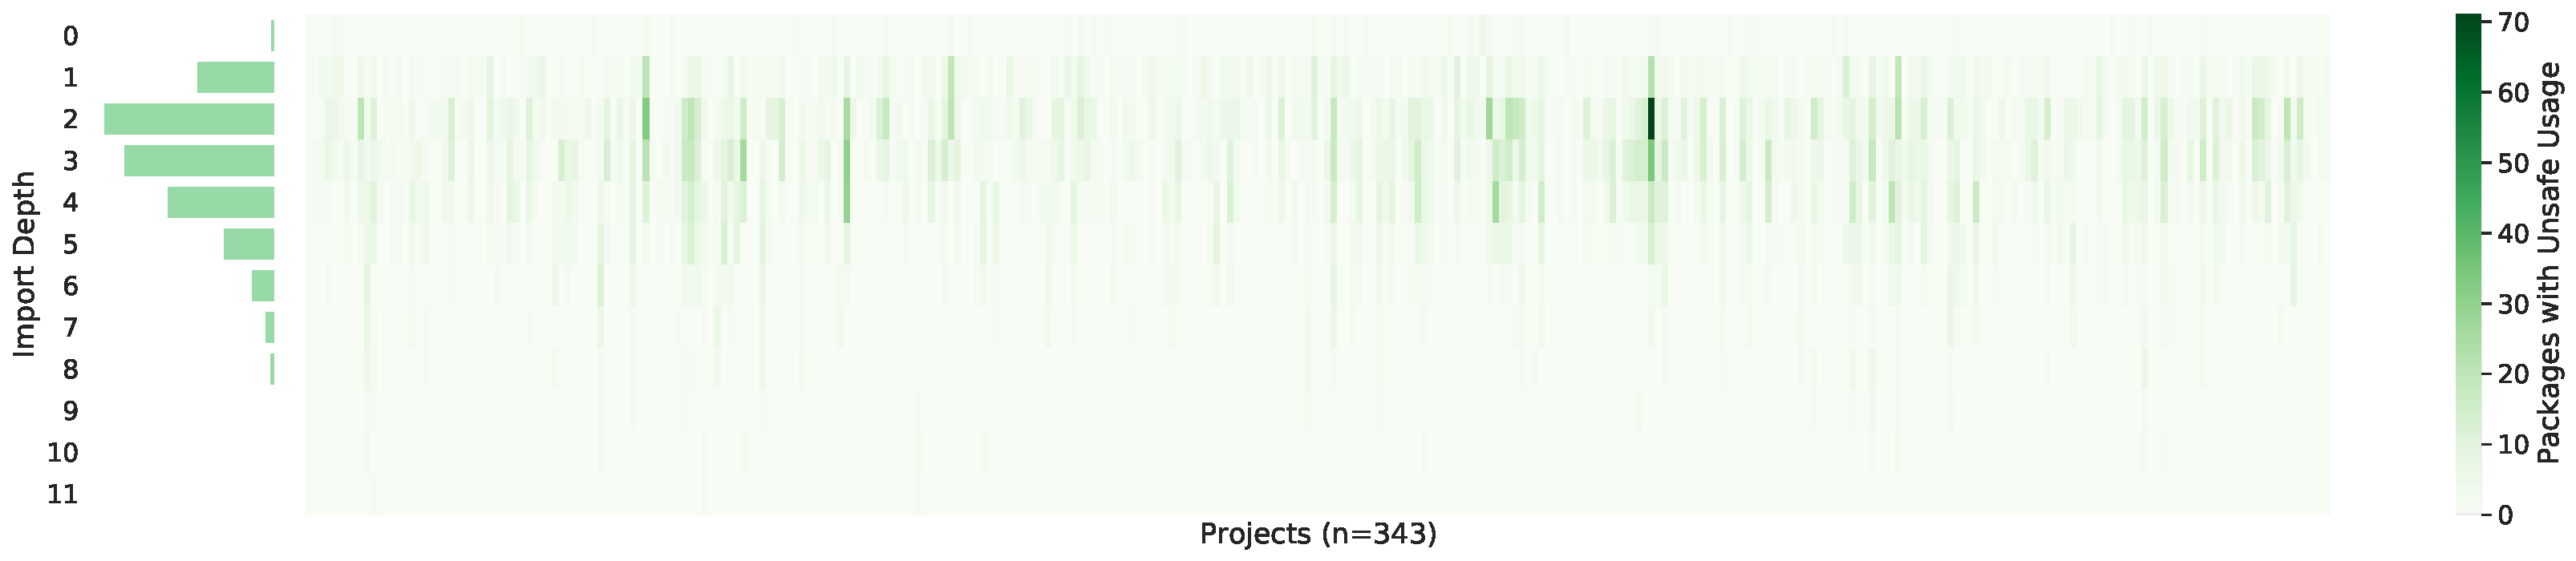
\includegraphics[width=\textwidth]{gfx/figures/unsafe-import-depth.pdf}
    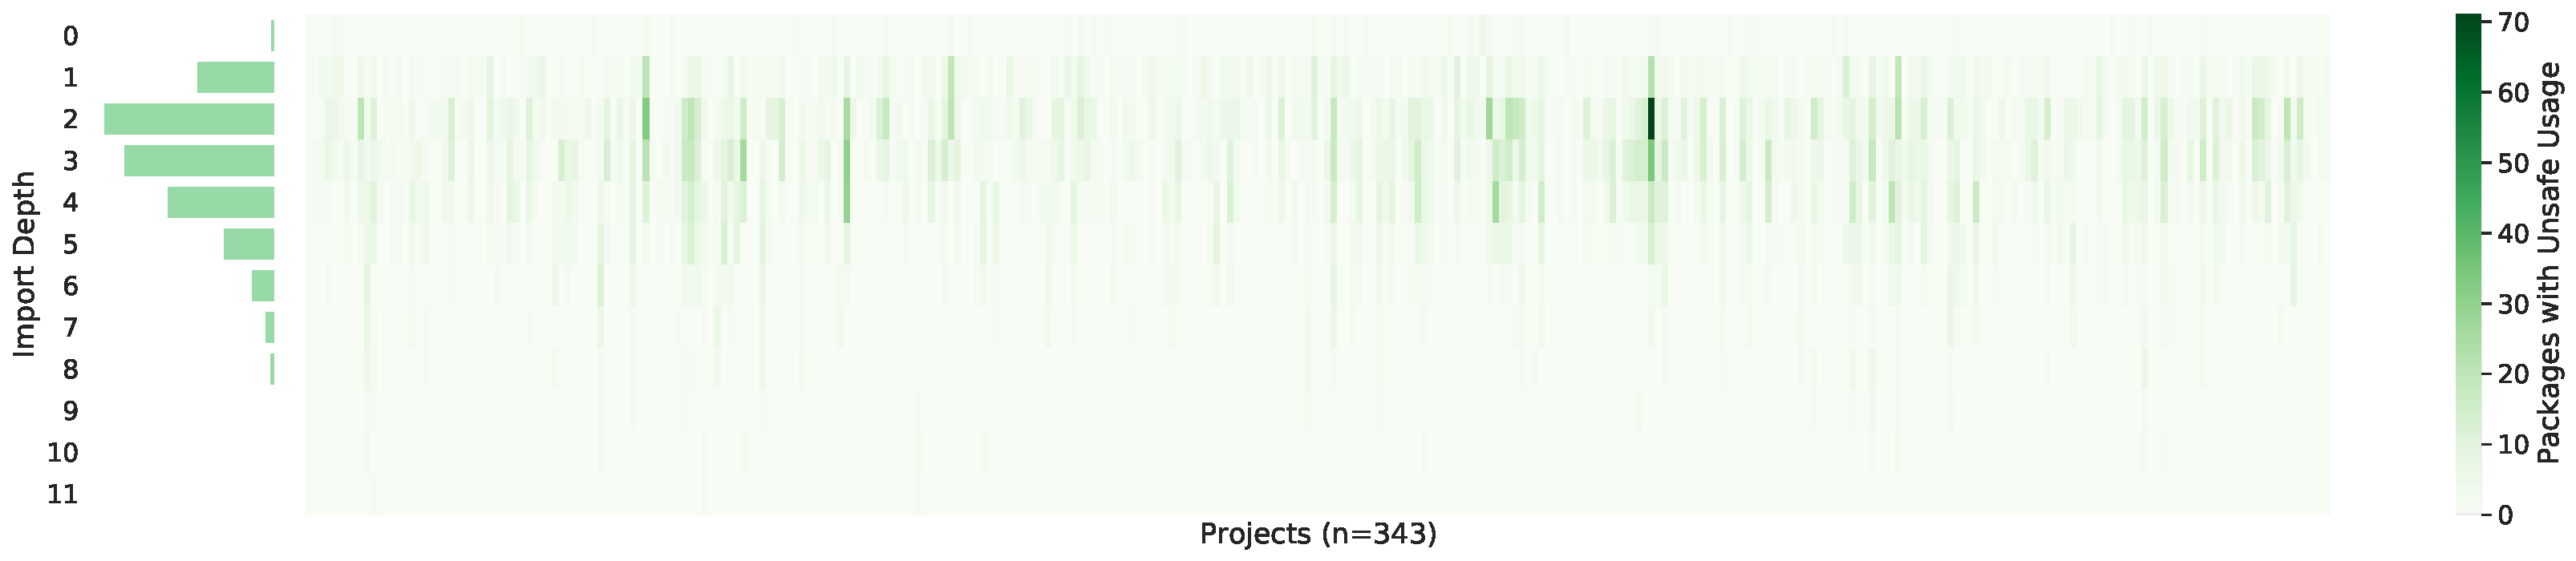
\includegraphics[width=.9\textwidth]{gfx/figures/unsafe-import-depth.pdf}
    \caption{Import Depth of Unsafe Packages. Unsafe packages are around a depth of \averageUnsafeImportDepth{} (sd=\stdUnsafeImportDepth{})}
    \label{fig:unsafe-import-depth}
    %\vspace{-10pt}
\end{figure*}




%% ---------------------------------------------------

\subsection{Data Set}

%For our evaluation, we created a data set of open-source Go code available on GitHub.
As our research is focused on open-source projects, we crawled the \initalProjs{} most-starred Go projects available on GitHub. 
To further understand the influence of dependencies, we then selected the applications supporting \textit{go modules}.
With the introduction of Go \checkNum{1.13}, \textit{go modules}\footnote{\url{https://blog.golang.org/using-go-modules}} are the official way to include dependencies.
Unfortunately, \withoutModules{} of the projects did not yet support Go modules.
Thus, we excluded them from our set.
Furthermore, \notCompiled{} projects that did not compile were also removed.
As a result, we ended up with \projsAnalyzed{} top-rated Go projects. % collected from GitHub.
These have between 72,988 and 3,075 stars, with an average of 7,860. % and median of 5,345. %, thus, this evaluation focuses on very popular projects.
%and save all findings into CSV files.



%% ---------------------------------------------------

\subsection{Unsafe Usages in Projects and Dependencies}
\label{sec:eval:unsafewild}

We used the Go tool chain to identify the root module of each project. 
This is the module defined by the top-level \textit{go.mod} file in the project.
Then we enumerated the dependencies of the project, and built the dependency tree.
For each package, we used \toolUsage{} to generate CSV reports of the found \unsafe{} usages.
Through these analyses we answer the research questions of how many projects use \unsafe{} either in their own code or dependencies (\ref{rq:prevalApp}), and how deep in the dependency tree are the most \unsafe{} code usages (\ref{rq:depsDepth}). 
By selecting only results from the project root modules, we can easily find out how many applications contain a first-hand use of \unsafe{} code.
Our data shows that \checkNum{131} (\checkNum{38.19\%}) projects have at least one \unsafe{} usage within the project code itself.
By looking closer at the imported packages, we see that \checkNum{3,388} of \checkNum{62,025} (\checkNum{5.46\%}) transitively imported packages use \unsafe{}. 
%Through filtering the imported packages, we find that \checkNum{33} of \checkNum{186} (\checkNum{17.74\%}) used standard library packages contain \unsafe{}.
%There are \checkNum{299} (\checkNum{87.17\%}) projects that have at least one direct dependency to a package that has $\geq 1$ unsafe dependency, however for this number we counted only packages belonging to the project's root module as first-party project code. \jl{Might be wrong numbers}
%If a project is split into several modules that all should be logically viewed as first-party project code, they will inflate this number.
There are \checkNum{312} (\checkNum{90.96\%}) projects that have at least one non-standard-library dependency with \unsafe{} usages somewhere in their dependency tree.
Since all projects include the Go runtime, which uses \unsafe{}, counting it as an \unsafe{} dependency would mean that \checkNum{100\%} of projects transitively include \unsafe{}.
We consider this to be less meaningful, as we assume the Go standard library is well audited and safer to use.

%\begin{tcolorbox}[boxsep=1pt, enlarge top by=5pt, title=Answer to \ref{rq:prevalDeps}]
\begin{tcolorbox}[boxsep=1pt, enlarge top by=5pt, title=Answer to \ref{rq:prevalApp}]
About \checkNum{38\%} of projects directly contain \unsafe{} usages.
Furthermore, about \checkNum{91\%} of projects transitively import at least one dependency that contains \unsafe{}.
\end{tcolorbox}

% Using this tree, we can identify the import depth as minimum depth in the tree for each package.
Figure~\ref{fig:unsafe-import-depth} shows the number of packages with at least one \unsafe{} usage by their depth in the dependency tree for every project on its own as a heatmap, alongside the distribution for all projects combined as bars on the left side.
It is evident that most packages with \unsafe{} are imported early in the dependency tree with an average depth of \averageUnsafeImportDepth{}~and a standard deviation of \stdUnsafeImportDepth{}.
This number is very similar to the overall average depth of imported packages (\averageGeneralImportDepth{}). %, regardless of whether they contain usages of \unsafe{}.
While the packages containing \unsafe{} can be manually found and evaluated, this process requires significant resources to handle the increasing number of packages introduced through each dependency. 
For developers only the first level of dependencies, the ones they added themselves, are really obvious.
On this level, \levelOneImportedUnsafePackagesCount{} out of \ImportedUnsafePackagesCount{} imported packages (\levelOneImportedUnsafePackagesShare{}) contain \unsafe{}.

\begin{tcolorbox}[boxsep=1pt, enlarge top by=5pt, title=Answer to \ref{rq:depsDepth}]
Most imported packages containing \unsafe{} usages are found around a depth of \checkNum{3} in the dependency tree.
\end{tcolorbox}



%% ---------------------------------------------------

\subsection{Types and Purpose of Unsafe in Practice}
\label{sec:eval:labeledData}

This section answers \ref{rq:distTypes} and \ref{rq:purpose}.
%This section answers the research questions which \unsafe{} keywords are used most (\ref{rq:distTypes}), as well as which \unsafe{} operations are used in practice for what purpose (\ref{rq:purpose}).
%
Figure~\ref{fig:unsafe-tokens-distribution} shows the distribution of the different \unsafe{} types in our data set.
Packages that are imported in different versions by the projects are counted once per version, as they might contain different \unsafe{} usages and coexist in the wild.
%We found various different usages of \unsafe{} in the analyzed projects, 
In our data set \textit{uintptr} and \textit{unsafe.Pointer} are used about equally often and are by far the most common with almost 100,000 findings. 
Next, \textit{unsafe.Sizeof} is still used a bit ($\sim 3,700$), while the other \unsafe{} types are rarely used~($< 1,000$).

\begin{tcolorbox}[boxsep=1pt, enlarge top by=5pt, title=Answer to \ref{rq:distTypes}]
In the wild, \textit{uintptr} and \textit{unsafe.Pointer} are orders of magnitude more common than other \unsafe{} usages.
\end{tcolorbox}

\begin{figure}[!t]
    \centering
    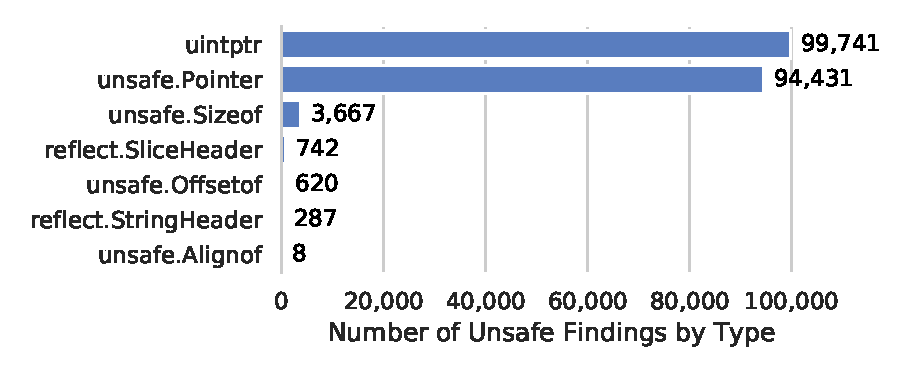
\includegraphics[width=0.43\textwidth]{assets/plots/distribution-unsafe-types.pdf}
    \caption{Distribution of different types of unsafe tokens}
    \label{fig:unsafe-tokens-distribution}
\end{figure}

To learn about the purpose and context in which \unsafe{} is used, we needed to manually analyze code.
Thus, we selected the top \checkNum{10} projects (Table~\ref{tbl:dataset-projects}) with the most \unsafe{} usages in non-standard library packages.
%These projects including the Git revision analyzed plus some additional data are shown in Table~\ref{tbl:dataset-projects}.
From these projects and all their transitive dependencies, we randomly sampled \checkNum{400} code snippets that were found in the \textit{standard library (std)} and \checkNum{1,000} snippets from the remaining packages (\textit{app}).
We define standard library code as all packages that are part of the Go standard library or the \textit{golang.org/x/sys} module, as the \textit{syscall} standard library package is deprecated in favor of this module\footnote{\url{https://golang.org/pkg/syscall}}.
We split the snippets into two groups to analyze if there is a difference between the official standard library and non-standard library code regarding the usage of \unsafe{}.
Then, we identify class labels in two dimensions: what is being done, and for what purpose. 
Finally, we manually analyze all \checkNum{1,400} code snippets and label them accordingly.
The results of this process are shown in Table~\ref{tbl:dataset-classes}.

\begin{table}[!t]
\vspace{2mm}

    \centering
    \caption{Projects selected for labeled data set}
    \label{tbl:dataset-projects}
    \begin{adjustbox}{max width=\textwidth}
    \begin{tabular}{llrrl}
        %\hline
        {} & \textbf{Name} &  \textbf{Stars} &  \textbf{Forks} &    \textbf{Revision} \\ \hline
        \rowcolor{verylightgray}
        1  &         kubernetes/kubernetes &  66,512 &  23,806 &  \texttt{fb9e1946b0} \\
        2  &                 elastic/beats &   8,852 &   3,207 &  \texttt{df6f2169c5} \\
        \rowcolor{verylightgray}
        3  &             gorgonia/gorgonia &   3,373 &    301 &  \texttt{5fb5944d4a} \\
        4  &              weaveworks/scope &   4,354 &    554 &  \texttt{bf90d56f0c} \\
        \rowcolor{verylightgray}
        5  &  mattermost/mattermost-server &  18,277 &   4,157 &  \texttt{e83cc7357c} \\
        6  &               rancher/rancher &  14,344 &   1,758 &  \texttt{56a464049e} \\
        \rowcolor{verylightgray}
        7  &                 cilium/cilium &   5,501 &    626 &  \texttt{9b0ae85b5f} \\
        8  &                     rook/rook &   7,208 &   1,472 &  \texttt{ff90fa7098} \\
        \rowcolor{verylightgray}
        9  &             containers/libpod &   4,549 &    539 &  \texttt{e8818ced80} \\
        10 &                       xo/usql &   5,871 &    195 &  \texttt{bdff722f7b} \\ %\hline
    \end{tabular}
    \end{adjustbox}
    %% reduce space after table for vspace tweaking
    \vspace{-10pt}
\end{table}
\begin{table*}[htp!]
    \centering
    \caption[Labeled unsafe.Pointer usages in application code (non standard library) and standard library samples]
        {Labeled unsafe.Pointer usages in application code (non standard library) and standard library samples~\newline \tiny ~\newline \footnotesize
        \underline{eff}: efficiency, \underline{ser}: (de)serialization, \underline{gen}: generics,
        \underline{no GC}: avoid garbage collection, \underline{atomic}: atomic operations,
        \underline{FFI}: foreign function interface, \underline{HE}: hide from escape analysis, \underline{layout}: memory layout control,
        \underline{types}: Go type system,
        \underline{reflect}: type reflection, \underline{unused}: declared but unused \tiny ~\newline}
    \label{tbl:dataset-classes}
    \begin{adjustbox}{max width=\textwidth}
    
    %% do not paste from notebook, local changes done!
\begin{tabular}{r|cc|cc|cc|cc|cc|cc|cc|cc|cc|cc|cc|cc}
                    & \multicolumn{2}{c|}{\textbf{eff}} & \multicolumn{2}{c|}{\textbf{ser}} & \multicolumn{2}{c|}{\textbf{gen}} & \multicolumn{2}{c|}{\textbf{no GC}} & \multicolumn{2}{c|}{\textbf{atomic}} & \multicolumn{2}{c|}{\textbf{FFI}} & \multicolumn{2}{c|}{\textbf{HE}} & \multicolumn{2}{c|}{\textbf{layout}} & \multicolumn{2}{c|}{\textbf{types}} & \multicolumn{2}{c|}{\textbf{reflect}} & \multicolumn{2}{c|}{\textbf{unused}} & \multicolumn{2}{c}{\textbf{total}} \\ %\hline
                    &  \textbf{app} &  \textbf{std} &  \textbf{app} &  \textbf{std} &  \textbf{app} &  \textbf{std} &   \textbf{app} &  \textbf{std} &    \textbf{app} &  \textbf{std} &  \textbf{app} &  \textbf{std} &  \textbf{app} &  \textbf{std} &    \textbf{app} &  \textbf{std} &   \textbf{app} &  \textbf{std} &     \textbf{app} &  \textbf{std} &    \textbf{app} &  \textbf{std} &   \textbf{app} &  \textbf{std} \\ \hline
                    
                    \textbf{cast} & 562 & 16 & 178 & 33 & 18 & & & & & & 24 & 6 && 2 & 3 & 13 & & 45 & 1 & & & & 786 & 115 \\ 
      %  cast-struct &  401 &    4 &   50 &    6 &    6 &      &       &      &        &      &    6 &    2 &      &    2 &        &    4 &       &   31 &         &      &        &      &   463 &   49 \\
%\rowcolor{verylightgray}
      %   cast-basic &   90 &    2 &   29 &    3 &    1 &      &       &      &        &      &    1 &    3 &      &      &      2 &    7 &       &    1 &         &      &        &      &   123 &   16 \\
      %  cast-header &   36 &    1 &    3 &      &    1 &      &       &      &        &      &      &      &      &      &        &      &       &    3 &         &      &        &      &    40 &    4 \\
%\rowcolor{verylightgray}
      %   cast-bytes &   22 &    1 &   81 &   11 &      &      &       &      &        &      &    1 &      &      &      &      1 &      &       &    1 &         &      &        &      &   105 &   13 \\
      % cast-pointer &   13 &    8 &   15 &   13 &   10 &      &       &      &        &      &   16 &    1 &      &      &        &    2 &       &    9 &       1 &      &        &      &    55 &   33 \\
\rowcolor{verylightgray}
      \textbf{memory-access} &    2 &    1 &    9 &      &      &      &       &      &        &      &      &    1 &      &      &      4 &    6 &       &    4 &         &      &        &      &    15 &   12 \\
 \textbf{pointer-arithmetic} &    7 &    2 &    6 &    1 &      &      &       &      &        &    1 &      &    3 &    1 &    2 &      3 &    8 &       &    9 &         &      &        &      &    17 &   26 \\
\rowcolor{verylightgray}
         \textbf{definition} &    4 &    1 &   23 &      &    2 &      &       &      &        &      &    4 &    5 &      &      &        &    9 &       &    8 &       6 &    3 &        &      &    39 &   26 \\
           \textbf{delegate} &    4 &      &   64 &      &    2 &      &       &      &     11 &    5 &   29 &   45 &      &    4 &        &   14 &       &    6 &         &    1 &        &      &   110 &   75 \\
\rowcolor{verylightgray}
            \textbf{syscall} &      &      &      &      &      &      &    17 &  138 &        &      &      &      &      &      &        &      &       &      &         &      &        &      &    17 &  138 \\
             \textbf{unused} &      &      &      &      &      &      &       &      &        &      &      &      &      &      &        &      &       &      &         &      &     16 &    8 &    16 &    8 \\ \hline
%\rowcolor{verylightgray}
                  \textbf{total} &  579 &   20 &  280 &   34 &   22 &    0 &    17 &  138 &     11 &    6 &   57 &   60 &    1 &    8 &     10 &   50 &     0 &   72 &       7 &    4 &     16 &    8 &  1000 &  400 \\
\end{tabular}

    \end{adjustbox}
        \vspace{-10pt}
\end{table*}

In the following, we outline the identified usage type classes describing what is being done in code.
The most prevalent are \textit{cast} operations from arbitrary types to other structs, basic Go types such as integers, slice/string headers, byte slices, or raw \textit{unsafe.Pointer} values. 
%The most prevalent are \textit{cast-struct}, \textit{cast-basic}, \textit{cast-header}, \textit{cast-bytes}, and \textit{cast-pointer}, which are all cast operations from arbitrary types to other arbitrary structs, basic Go types such as integers, slice or string headers, byte slices, or raw \textit{unsafe.Pointer} values.
The \textit{memory-access} class is applied where \textit{unsafe.Pointer} values are dereferenced, used to manipulate corresponding memory or for comparison with another address.
\textit{Pointer-arithmetic} denotes usages of \unsafe{} to do some form of arithmetic manipulation of addresses, such as advancing an array.
\textit{Definition} groups usages where a field or method of type \textit{unsafe.Pointer} is declared for later usage.
\textit{Delegate} are instances where \unsafe{} is only needed in a function to pass it along to another function requiring a parameter of type \textit{unsafe.Pointer}. 
Thus, the need to use \unsafe{} is actually located elsewhere.
\textit{Syscall} are calls using the Go \textit{syscall} package or \textit{golang.org/x/sys} module.
As the name suggests, \textit{unused} is a class of occurrences that are not actually used in the analyzed code, e.g., dead code or unused parameters.

Our identified purpose classes, providing hints on why \unsafe{} is used, are described in the following.
\textit{Efficiency} includes cases where \unsafe{} is used only for the aim to improve time or space efficiency of the code.
The \textit{serialization} class contains (un)marshalling and (de)serialization operations such as in-place casts from complex types to bytes.
\textit{Generics} applies when \unsafe{} is used to build functionality that would otherwise be solved with generics if they were available in Go.
Samples in the \textit{avoid garbage collection} class are used to tell the Go compiler to not free a value while it is used, e.g., by a function written in assembly.
The \textit{atomic operations} class contains usages of the \textit{atomic} API which expects \unsafe{} for some functions.
The \textit{foreign function interface (FFI)} class contains interoperability with C code (CGo), and calling  functions that expect their parameters as \unsafe{} pointers.
\textit{Hide from escape analysis} includes the pattern described earlier (Listing~\ref{lst:unsafe-ex-escape-analysis}) to break the escape analysis chain.
The \textit{memory layout control} class contains code used for low-level memory management.
\textit{Types} snippets are used by the standard library to implement the Go type system.
\textit{Reflect} includes instances of type reflection and re-implementations of some types of the \textit{reflect} package, e.g., using \textit{unsafe.Pointer} instead of \textit{uintptr} for slice headers.
Again, \textit{unused} is a class of unused occurrences.

%Among the \checkNum{1,400} labeled snippets, \checkNum{683} are located in automatically generated code.
%It might be safe to assume that generated code is less dangerous, however, as bugs in the code generator can have very serious effects of scale, we included them in the study nonetheless.

Using \unsafe{} for the sake of efficiency is the most prevalent motivation to use \unsafe{} in the wild covering \checkNum{58\%} in application code, whereas it is only used for this purpose in \checkNum{5\%} of the cases in std. 
From these, \checkNum{97\%} resp. \checkNum{80\%} are achieved by casting different types. 
The second biggest reason to use \unsafe{} in app is to perform some form of (de)serialization, accounting for \checkNum{28\%}.
%Interestingly, we observe efficiency improvements for \checkNum{4\%} and \checkNum{58\%} of the usages for the standard library and the remaining libraries, respectively.
For the standard library, the most relevant motivation is avoiding garbage collection with \checkNum{35\%}, whereas this is only used in \checkNum{2\%} of the usages in the app sample.
Furthermore, in std type \checkNum{18\%}, FFI \checkNum{15\%} and memory layout \checkNum{13\%} related \unsafe{} usages are rather common.
Both subsets share that hiding from escape analysis with \checkNum{0.1\%} (\textit{app}) and \checkNum{2\%} (\textit{std}) and using \unsafe{} for reflection with \checkNum{1\%} (both) are rare.
%Another interesting observation is that there seem to be two main motivations which occur only for the standard- or 3rd party libraries respectively. 
%Only the standard library makes use of \unsafe{} to implement types being \checkNum{5\%} of the analyzed code snippets. 
%All usages (\checkNum{2\%}) to solve the missing generics functionality in Go are within 3rd party libraries. 
Implementation of generics functionality which is currently missing in Go is only done in few samples (\checkNum{2\%}), although some of the findings in the serialization class could alternatively be achieved with generics as well.

%It is obvious that most of the \unsafe{} found in the wild is used to improve efficiency by casting different types in place, or for fast (un)marshalling operations that would otherwise need either reflection or support for generics.
%Furthermore, \unsafe{} is required to call some functions that expect it, such as atomic operations or certain \textit{FFI} functions.
%The standard library makes extensive use of \unsafe{} to implement types and memory management.
%Hiding values from escape analysis on purpose is done rarely.

\begin{tcolorbox}[boxsep=1pt, enlarge top by=5pt, title=Answer to \ref{rq:purpose}]
\checkNum{More than half} of the \unsafe{} usages in projects and 3rd party libraries are to improve efficiency via \unsafe{} casts.
In the Go standard library, \checkNum{every third} use of \unsafe{} is to avoid garbage collection. 
\end{tcolorbox}


\subsection{Vulnerable Usages}
\label{sec:discussion}
Looking at the study results, we see that \unsafe{} is used consistently and wide-spread in the most popular open-source Go projects.
One might argue that the \new{usages}
%patterns 
found by \toolUsage{} are only minor annoyances, not severe or would require a manual case-to-case inspection. 
\new{Still, t}he exploitability of several of these %patterns 
\new{usages}
was discussed in \new{Section~\ref{sec:appr:vulnerabilites} with a reference to \checkNum{six} proof-of-concept exploits} that we developed\new{.}
%, clearly 
\new{This c}learly \new{shows} that it is indeed possible to use the memory corruptions to one's advantage.
However, not all \unsafe{} usages contain a vulnerability. 
As already discussed, we implemented more specific checks for \new{two} %some of our 
patterns known to be problematic in \toolSA{} \new{(Section~\ref{sec:appr:toolSA})}.
\new{With it, three of the proof-of-concept exploits are mitigated, leaving the others which are much harder to detect statically for future work.}
The application of \toolSA{} to our data set revealed more than \numberBugsFixed{} \new{insecure usages of \unsafe{}}
%bugs 
in different projects.
Based on the results, we submitted so far \numberPRs{} pull requests to fix the\new{se usages.} 
%found bugs. %, which focuses on a subset of vulnerable code patterns.
By now, \numberPRsMerged{} have already been reviewed, acknowledged, and accepted by the corresponding project maintainers.